\chapter{第十三次作业}

    \begin{homework}[6pts]
        用图解法求解下列线性规划问题,并指出问题是否有唯一最优解、无穷多最优解、无界解还是无可行解?
        \begin{flalign*}
            \max \quad&z=2x_1+3x_2 \\
            \st \quad&x_1+2x_2\leq 8 \\
            &2x_1+x_2\geq 1 \\
            &x_2\leq 3 \\
            &x_1,x_2\geq 0
        \end{flalign*}
    \end{homework}

    \begin{solution}
        图像如下图所示:

        \begin{center}
            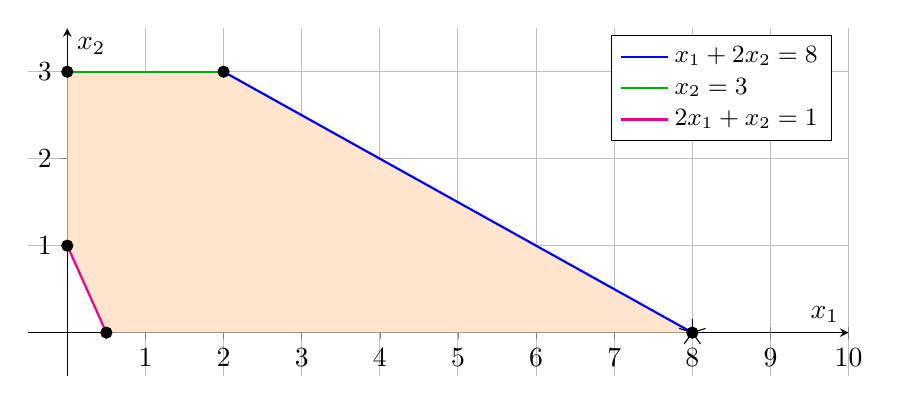
\begin{tikzpicture}
                \begin{axis}[
                    width=12cm,
                    height=6cm,
                    axis lines=middle,
                    xmin=-0.5,xmax=10,
                    ymin=-0.5,ymax=3.5,
                    xlabel={$x_1$},
                    ylabel={$x_2$},
                    grid=both,
                    legend cell align=left,
                    legend style={font=\small,at={(0.98,0.98)},anchor=north east},
                    clip=false]

                    \addplot[
                      draw=none,
                      fill=orange!20,
                      forget plot
                    ] coordinates{
                      (0.5,0)(8,0)(2,3)(0,3)(0,1)
                    } -- cycle;

                    \addplot[
                      domain=2:8,
                      samples=2,
                      thick,
                      color=blue
                    ]{(8-x)/2};
                    \addlegendentry{$x_{1}+2x_{2}=8$}

                    \addplot[
                      domain=0:2,
                      samples=2,
                      thick,
                      color=green!70!black
                    ]{3};
                    \addlegendentry{$x_{2}=3$}

                    \addplot[
                      domain=0:0.5,
                      samples=2,
                      thick,
                      color=magenta
                    ]{1-2*x};
                    \addlegendentry{$2x_{1}+x_{2}=1$}

                    \addplot[only marks,mark=*] coordinates{
                    (0.5,0) (8,0) (2,3) (0,3) (0,1)
                    };

                    \addplot[only marks,mark=star,mark size=5,fill=red] coordinates {(8,0)};

                \end{axis}
            \end{tikzpicture}
        \end{center}

        直线对应约束条件,橙色区域为可行域。可行基解为$(0.5,0),(8,0),(2,3),(0,3),(0,1)$,

        对应值为$1,16,13,9,3$,因此最优解为$(8,0)$,对应目标函数值为$16$,存在唯一最优解。
    \end{solution}

    \begin{homework}[6pts]
        将下列线性规划问题化为标准形式,并列出初始单纯形表.
        \begin{flalign*}
            \min \quad&z=-x_1+2x_2-3x_3+2x_4 \\
            \st \quad& 4x_1-x_2+2x_3-x_4=-2 \\
            &x_1+x_2-x_3+2x_4\leq 14 \\
            &-2x_1+3x_2+x_3-x_4\geq 2 \\
            & x_1,x_2,x_3\geq 0, x_4\,\text{无约束}
        \end{flalign*}
    \end{homework}

    \begin{solution}
        令$x_4=x_5-x_6,x_5,x_6\geq 0$,对后两个不等式约束添加松弛变量$x_7,x_8$,则标准形式为:
        \begin{flalign*}
            \max \quad&z=x_1-2x_2+3x_3-2x_5+2x_6 \\
            \st \quad& -4x_1+x_2-2x_3+x_5-x_6=2 \\
            &x_1+x_2-x_3+2x_5-2x_6+x_7=14 \\
            &-2x_1+3x_2+x_3-x_5+x_6-x_8=2 \\
            & x_1,x_2,x_3, x_5,x_6,x_7,x_8\geq 0
        \end{flalign*}

        容易得到一组初始基可行解为$(x_1,x_2,x_3,x_5,x_6,x_7,x_8)=(0,2,0,0,0,12,4)$,

        对应目标函数值为$-4$,初始单纯形表如下:

        \begin{table}[H]
            \centering
            \begin{tabular}{|c|c|c|c|c|c|c|c|c|c|}
                \hline
                \multicolumn{3}{|c|}{$c_j\rightarrow$} & $1$ & $-2$ & $3$ & $-2$ & $2$ & $0$ & $0$  \\
                \hline
                $c_B$ & $x_B$ & $b$ & $x_1$ & $x_2$ & $x_3$ & $x_5$ & $x_6$ & $x_7$ & $x_8$ \\
                \hline
                $-2 $& $x_2$ & $2$ & $-4$ & $1$ & $-2$ & $1$ & $-1$ & $0$ & $0$\\
                \hline
                $0$ & $x_7$ & $12$ & $1$ & $1$ & $-1$ & $2$ & $-2$ & $1$ & $0$\\
                \hline
                $0$ & $x_8$ & $4$ & $-2$ & $3$ & $1$ & $-1$ & $1$ & $0$ & $-1$\\
                \hline
                \multicolumn{3}{|c|}{$\sigma_j$} & $-7$ & $0$ & $-1$ & $0$ & $0$ & $0$ & $0$\\
                \hline
            \end{tabular}
        \end{table}
    \end{solution}

    \begin{homework}[6pts]
        求下列线性规划问题中满足约束条件的所有基解,并指出哪些是基可行解,并代入目标函数,确定哪一个是最优解。
        \begin{flalign*}
            \max \quad& z=2x_1-x_2+3x_3+2x_4 \\
            \st \quad& 2x_1+3x_2-x_3-4x_4 = 8 \\
            &x_1-2x_2+6x_3-7x_4 = -3 \\
            &x_1,x_2,x_3,x_4\geq 0
        \end{flalign*}
    \end{homework}

    \begin{solution}
        有$2$个等式约束和$4$个变量,因此需要令除基变量的$2$个变量为$0$,以下为结果:

        \begin{table}[H]
            \centering
            \begin{tabular}{|c|c|c|c|c|}
                \hline
                基变量 & 解向量 & 是否可行 & 目标函数值 \\
                \hline
                $x_1,x_2$ & $(1,2,0,0)$ & 是 & $0$ \\
                \hline
                $x_1,x_3$ & $(\tfrac{45}{13},0,-\tfrac{14}{13},0)$ & 否 & N/A \\
                \hline
                $x_1,x_4$ & $(\tfrac{34}5,0,0,\tfrac75)$ & 是 & $\tfrac{82}5$ \\
                \hline
                $x_2,x_3$ & $(0,\tfrac{45}{16},\tfrac7{16},0)$ & 是 & $-\tfrac32$ \\
                \hline
                $x_2,x_4$ & $(0,\tfrac{68}{29},0,-\tfrac7{29})$ & 否 & N/A \\
                \hline
                $x_2,x_3$ & $(0,0,-\tfrac{68}{31},-\tfrac{45}{31})$ & 否 & N/A \\
                \hline
            \end{tabular}
        \end{table}
    \end{solution}

    \begin{homework}[6pts]
        用单纯形方法求解以下线性规划问题:
        \begin{flalign*}
            \max \quad& z=3x_1-2x_2+5x_3 \\
            \st \quad &3x_1+2x_3\leq 13 \\
            & x_2+3x_3\leq 17 \\
            &2x_1+x_2+x_3\leq 13 \\
            &x_1,x_2,x_3\geq0
        \end{flalign*}
    \end{homework}

    \begin{solution}
        对约束条件添加松弛变量$x_4,x_5,x_6$,则标准形式为:
        \begin{flalign*}
            \max \quad& z=3x_1-2x_2+5x_3 \\
            \st \quad &3x_1+2x_3+x_4=13 \\
            & x_2+3x_3+x_5=17 \\
            &2x_1+x_2+x_3+x_6=13 \\
            &x_1,x_2,x_3,x_4,x_5,x_6\geq 0
        \end{flalign*}

        一组初始基可行解为$(x_1,x_2,x_3,x_4,x_5,x_6)=(0,0,0,13,17,13)$,初始单纯形表如下:

        \begin{table}[H]
            \centering
            \begin{tabular}{|c|c|c|c|c|c|c|c|c|}
                \hline
                \multicolumn{3}{|c|}{$c_j\rightarrow$} & $3$ & $-2$ & $5$ & $0$ & $0$ & $0$ \\
                \hline
                $c_B$ & $x_B$ & $b$ & $x_1$ & $x_2$ & $x_3$ & $x_4$ & $x_5$ & $x_6$ \\
                \hline
                $0$& $x_4$ & $13$ & $3$ & $0$ & $2$ & $1$ & $0$ & $0$\\
                \hline
                $0$& $x_5$ & $17$ & $0$ & $1$ & $3$ & $0$ & $1$ & $0$\\
                \hline
                $0$& $x_6$ & $13$ & $2$ & $1$ & $1$ & $0$ & $0$ & $1$\\
                \hline
                \multicolumn{3}{|c|}{$\sigma_j$} & $3$ & $-2$ & $5$ & $0$ & $0$ & $0$\\
                \hline
            \end{tabular}
        \end{table}

        以下进行单纯形表迭代:

        \begin{table}[H]
            \centering
            \begin{tabular}{|c|c|c|c|c|c|c|c|c|}
                \hline
                \multicolumn{3}{|c|}{$c_j\rightarrow$} & $3$ & $-2$ & $5$ & $0$ & $0$ & $0$ \\
                \hline
                $c_B$ & $x_B$ & $b$ & $x_1$ & $x_2$ & $x_3$ & $x_4$ & $x_5$ & $x_6$ \\
                \hline
                $0$& $x_4$ & $\tfrac{5}{3}$ & $3$ & $-\tfrac{2}{3}$ & $0$ & $1$ & $-\tfrac{2}{3}$ & $0$\\
                \hline
                $5$& $x_3$ & $\tfrac{17}{3}$ & $0$ & $\tfrac{1}{3}$ & $1$ & $0$ & $\tfrac{1}{3}$ & $0$\\
                \hline
                $0$& $x_6$ & $\tfrac{22}{3}$ & $2$ & $\tfrac{2}{3}$ & $0$ & $0$ & $-\tfrac{1}{3}$ & $1$\\
                \hline
                \multicolumn{3}{|c|}{$\sigma_j$} & $3$ & $-\tfrac{11}{3}$ & $0$ & $0$ & $-\tfrac{5}{3}$ & $0$\\
                \hline
            \end{tabular}
        \end{table}

        \begin{table}[H]
            \centering
            \begin{tabular}{|c|c|c|c|c|c|c|c|c|}
                \hline
                \multicolumn{3}{|c|}{$c_j\rightarrow$} & $3$ & $-2$ & $5$ & $0$ & $0$ & $0$ \\
                \hline
                $c_B$ & $x_B$ & $b$ & $x_1$ & $x_2$ & $x_3$ & $x_4$ & $x_5$ & $x_6$ \\
                \hline
                $3$& $x_1$ & $\tfrac59$ & $1$ & $-\tfrac29$ & $0$ & $\tfrac13$ & $-\tfrac29$ & $0$\\
                \hline
                $5$& $x_3$ & $\tfrac{17}3$ & $0$ & $\tfrac13$ & $1$ & $0$ & $\tfrac13$ & $0$\\
                \hline
                $0$& $x_6$ & $\tfrac{56}9$ & $0$ & $\tfrac{10}9$ & $0$ & $-\tfrac23$ & $\tfrac19$ & $1$\\
                \hline
                \multicolumn{3}{|c|}{$\sigma_j$} & $0$ & $-3$ & $0$ & $-1$ & $-1$ & $0$\\
                \hline
            \end{tabular}
        \end{table}

        因此最优解为$\left(\dfrac59,0,\dfrac{17}3,0,0,\dfrac{56}9\right)$,对应目标函数值为$30$。
    \end{solution}

    \begin{homework}[6pts]
        用大M法求解下列线性规划问题:
        \begin{flalign*}
            \min \quad& z=3x_1-x_2 \\
            \st \quad& 3x_1+x_2\geq 3 \\
            &2x_1-3x_2\geq 1\\
            &x_1,x_2\geq 0
        \end{flalign*}
    \end{homework}

    \begin{solution}
        对约束条件添加松弛变量$x_3,x_4$,并添加人工变量$x_5,x_6$,则标准形式为:
        \begin{flalign*}
            \max \quad& z=-3x_1+x_2-Mx_5-Mx_6 \\
            \st \quad& 3x_1+x_2-x_3+x_5=3 \\
            &2x_1-3x_2-x_4+x_6=1 \\
            & x_1,x_2,x_3,x_4,x_5,x_6\geq 0
        \end{flalign*}

        初始基可行解为$(x_1,x_2,x_3,x_4,x_5,x_6)=(0,0,0,0,3,1)$,初始单纯形表如下:

        \begin{table}[H]
            \centering
            \begin{tabular}{|c|c|c|c|c|c|c|c|c|}
                \hline
                \multicolumn{3}{|c|}{$c_j\rightarrow$} & $-3$ & $1$ & $0$ & $0$ & $-M$ & $0$ \\
                \hline
                $c_B$ & $x_B$ & $b$ & $x_1$ & $x_2$ & $x_3$ & $x_4$ & $x_5$ & $x_6$ \\
                \hline
                $-M$& $x_5$ & $3$ & $3$ & $1$ & $-1$ & $0$ & $1$ & $0$\\
                \hline
                $-M$& $x_6$ & $1$ & $2$ & $-3$ & $0$ & $-1$ & $0$ & $1$\\
                \hline
                \multicolumn{3}{|c|}{$\sigma_j$} & $5M-3$ & $1-2M$ & $-M$ & $-M$ & $0$ & $0$\\
                \hline
            \end{tabular}
        \end{table}

        以下进行单纯形表迭代:

        \begin{table}[H]
            \centering
            \begin{tabular}{|c|c|c|c|c|c|c|c|c|}
                \hline
                \multicolumn{3}{|c|}{$c_j\rightarrow$} & $-3$ & $1$ & $0$ & $0$ & $-M$ & $0$ \\
                \hline
                $c_B$ & $x_B$ & $b$ & $x_1$ & $x_2$ & $x_3$ & $x_4$ & $x_5$ & $x_6$ \\
                \hline
                $-M$& $x_5$ & $\tfrac32$ & $0$ & $\tfrac{11}2$ & $-1$ & $\tfrac32$ & $1$ & $-\tfrac32$\\
                \hline
                $-3$& $x_1$ & $\tfrac12$ & $1$ & $-\tfrac32$ & $0$ & $-\tfrac12$ & $0$ & $\tfrac12$\\
                \hline
                \multicolumn{3}{|c|}{$\sigma_j$} & $0$ & $\tfrac{11M-7}2$ & $-M$ & $\tfrac{3M}2$ & $0$ & $\tfrac{3-5M}2$\\
                \hline
            \end{tabular}
        \end{table}

        \begin{table}[H]
            \centering
            \begin{tabular}{|c|c|c|c|c|c|c|c|c|}
                \hline
                \multicolumn{3}{|c|}{$c_j\rightarrow$} & $-3$ & $1$ & $0$ & $0$ & $-M$ & $0$ \\
                \hline
                $c_B$ & $x_B$ & $b$ & $x_1$ & $x_2$ & $x_3$ & $x_4$ & $x_5$ & $x_6$ \\
                \hline
                $1$& $x_2$ & $\tfrac3{11}$ & $0$ & $1$ & $-\tfrac2{11}$ & $\tfrac3{11}$ & $\tfrac2{11}$ & $-\tfrac3{11}$\\
                \hline
                $-3$& $x_1$ & $\tfrac{10}{11}$ & $1$ & $0$ & $-\tfrac3{11}$ & $-\tfrac1{11}$ & $\tfrac3{11}$ & $\tfrac1{11}$\\
                \hline
                \multicolumn{3}{|c|}{$\sigma_j$} & $0$ & $0$ & $-\tfrac7{11}$ & $-\tfrac6{11}$ & $\tfrac7{11}-M$ & $\tfrac6{11}-M$ \\
                \hline
            \end{tabular}
        \end{table}

        因此最优解为$\left(\dfrac{10}{11},\dfrac{3}{11},0,0,0,0\right)$,对应目标函数值为$-\dfrac{27}{11}$。
    \end{solution}

    \begin{homework}[6pts]
        分别用最速下降法与牛顿法求函数$f(x)=x_1^2-x_1 x_2
        +x_2^2+x_1 x_3+x_3^2-2x_1+4x_2+2x_3-2, x=(x_1,x_2,x_3)^{\top}\in\mathbb{R}^3$的极小点, 初始点$x_0=(0,0,0)^{\top}$,要求:
        \begin{enumerate}
            \item 最速下降法进行$2$次迭代, 并验证相邻两步的搜索方向正交;
            \item 牛顿法进行1次迭代。
        \end{enumerate}
    \end{homework}

    \begin{solution}
        $\nabla f=(2x_1-x_2+x_3-2,-x_1+2x_2+4,x_1+2x_3+2)^{\top},\nabla^2 f=\begin{bmatrix}2&-1&1\\-1&2&0\\1&0&2\end{bmatrix}$。

        对于最速下降法,初始点为$x_0=(0,0,0)^{\top},d_0=\nabla f(x_0)=(-2,4,2)^{\top}$,

        $\alpha_0=\argmin_{\alpha}f(x_0+\alpha d_0)=\argmin_{\alpha}(28\alpha^2-24\alpha-2)=\dfrac37$,

        $x_1=x_0+\alpha_0 d_0=\left(\dfrac67,-\dfrac{12}7,-\dfrac67\right)^{\top},d_1=\nabla f(x_1)=\left(\dfrac47,-\dfrac27,\dfrac87\right)^{\top},\langle d_0,d_1\rangle=0$,

        $\alpha_1=-\dfrac{\nabla f(x_1)^{\top}d_1}{d_1^{\top}\nabla^2 f(x_1)d_1}=\dfrac{21}{62},x_2=x_1+\alpha_1 d_1=\left(\dfrac{144}{217},-\dfrac{351}{217},-\dfrac{270}{217}\right)^{\top}$,

        对于牛顿法,$x_1=x_0-\nabla^2 f(x_0)^{-1}\nabla f(x_0)=\left(1,-\dfrac32,\dfrac32\right)^{\top}$,

        由于$\nabla^2 f\succ 0,\nabla f(x)=0$时$x^*=\left(1,-\dfrac32,\dfrac32\right)^{\top}$,有$x^*$为全局最优解,$f(x^*)=-\dfrac{15}2$。
    \end{solution}